\documentclass[../main.tex]{subfiles}

\begin{document}
	\section{Thermal Properties of Matter}	
	\begin{preamb}
		Matter has some properties when it comes to heat. These preambles are also getting difficult to write because I'm running out of ideas.
	\end{preamb}
	
	\subsection{Heat Energy}
	
	\pdef{Zeroth Law of Thermodynamics}{(\textit{This isn't in syllabus.}) The zeroth law of thermodynamics states that if object A, B, and C are in thermal contact with each other, and if the temperature of object A is equal to that of B, and the temperature of object B is equal to that of C, then the temperature of object A must equal to that of C.}
	\begin{center}
		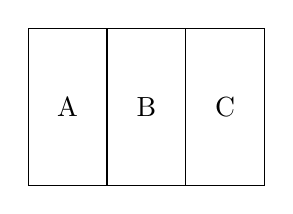
\begin{tikzpicture}
			\draw (0,0) rectangle (1,2) node[pos=.5] {A};
			\draw (1,0) rectangle (2,2) node[pos=.5] {B};
			\draw (2,0) rectangle (3,2) node[pos=.5] {C};
		\end{tikzpicture}
	\end{center}
	if \(T_A = T_B\) and \(T_B = T_C\) then
	\[ T_A = T_B = T_C \]
	
	\pdef{Heat Capacity}{Heat capacity \( C \) is the amount of heat energy required to raise the temperature of an object by \SI{1}{\kelvin}. Its relationship can be expressed as \[ \Delta Q = C \Delta T\] The SI unit of heat capacity is joule per kelvin [\si{\joule \per \kelvin}].}
	
	\pdef{Specific Heat Capacity}{Specific heat capacity \( c \) is the amount of heat energy required to raise the temperature of a unit mass of an object by \SI{1}{\kelvin}. Its relationship can be expressed as \[ \Delta Q = mc \Delta T\] The SI unit of heat capacity is joule per kelvin per kilogram [\si{\joule \per \kelvin \per \kilo\gram }].}
	
	\pdef{Latent Heat}{Latent heat is the energy released or absorbed by a substance during a change of state, without a change in its temperature. In general, \[ Q_{f/v} = ml_{f/v} \] where \(l_{f/v}\) is the specific latent heat of fusion/vaporisation, the heat energy required to melt or freeze/vaporise or condense a unit mass. The SI unit of specific latent heat is joule per kilogram [\si{\joule \per \kilo\gram}].}
	
	\subsection{Vaporisation}
	
	\pdef{Evaporation}{Evaporation is the process whereby a liquid vaporises at the surface because it has the energy equal or more than that of the latent heat of vaporisation, allowing it to escape into the atmosphere.}
	Evaporation can happen at any temperature.
	
	\pdef{Boiling}{Boiling is the process where a liquid reaches boiling point and the particles have enough energy to vaporise.}
	Boiling only happens at boiling point.
\end{document}
